\documentclass{classes/resume}

\title{
	プラスチック製品の部品整列作業自動化についての研究
}

\author{
	信州大学大学院 総合理工学研究科 繊維学専攻 機械・ロボット学分野 23FS307B 鎌田涼介
}

\begin{document}
\maketitle
\section{緒言}
昨今では工場での人材不足の解決や工場での作業の効率
化を目的とした作業の自動化が進んでいる.そこで注目さ
れている技術として,機械学習による画像解析を利用した
部品の品質検査や,ロボットによる部品の搬送などがある.
これらの技術を利用した自動化により,工場の生産性の向
上や人材の不足の解消が期待されている.
しかし依然として,人間によって行われている作業も数
多く存在する.本研究の目的はそのような実際の工場にお
いて問題になっている,プラスチック製品の部品整列作業
を自動化することである.

現在の工場では2種類の部品を表裏を区
別して並べる作業が人によって行われている.

問題点として手作業で行うため作業時間に限度があることや,部品1つ1つの単価が安く,人件費がかけられないことが挙げられる.

これらの問題点を解決するために本研究では作業工程を以
下の3つに分けて自動化を行う.
\vspace*{-0.5\zh}
\begin{itemize}
    \item 部品の表裏の判別
    \item 部品を並べる
    \item 正しい向きに部品を反転させる
\end{itemize}
\vspace*{-0.5\zh}

本機構は大きく分けて(1) 部品を1つずつ排出する機構,(2) 部品の向きを変える機構,(3) 部品の表裏判別,(4) 部品をスタックさせる機構,(5) 部品を反転させる機構で構成されている.


%実際の工程順に手法を説明する
\section{提案手法}
\subsection{1つずつ排出する機構}
    今回研究対象となる部品は直径約65 mm と大きい部品なので振動によるパーツフィーダを用いようとすると,パーツフィーダが大型化することになる\cite{ref:フィーダー}.
    そこで本研究ではパーツフィーダーを用いずに,部品を1つずつ排出する機構を考えた.
    この段階では裏表の区別なく部品を排出することを目的とする.

    その機構をFig.\ref{fig:rotationpart}に示す.この機構は穴の円周の大きさを部品の直径に合わせて設計することで,部品を1つずつ排出することができる.真ん中の部分が回転することで部品を1つずつ回転体の穴に嵌め合わせ,そこの部分に空いている部品1つ分の穴から排出する.

    排出された部品はFig.\ref{fig:detectarea}の機構によってスタックされる.

    \begin{figure}[b]
        \centering
        \begin{minipage}[t]{0.45\linewidth}
            \centering
            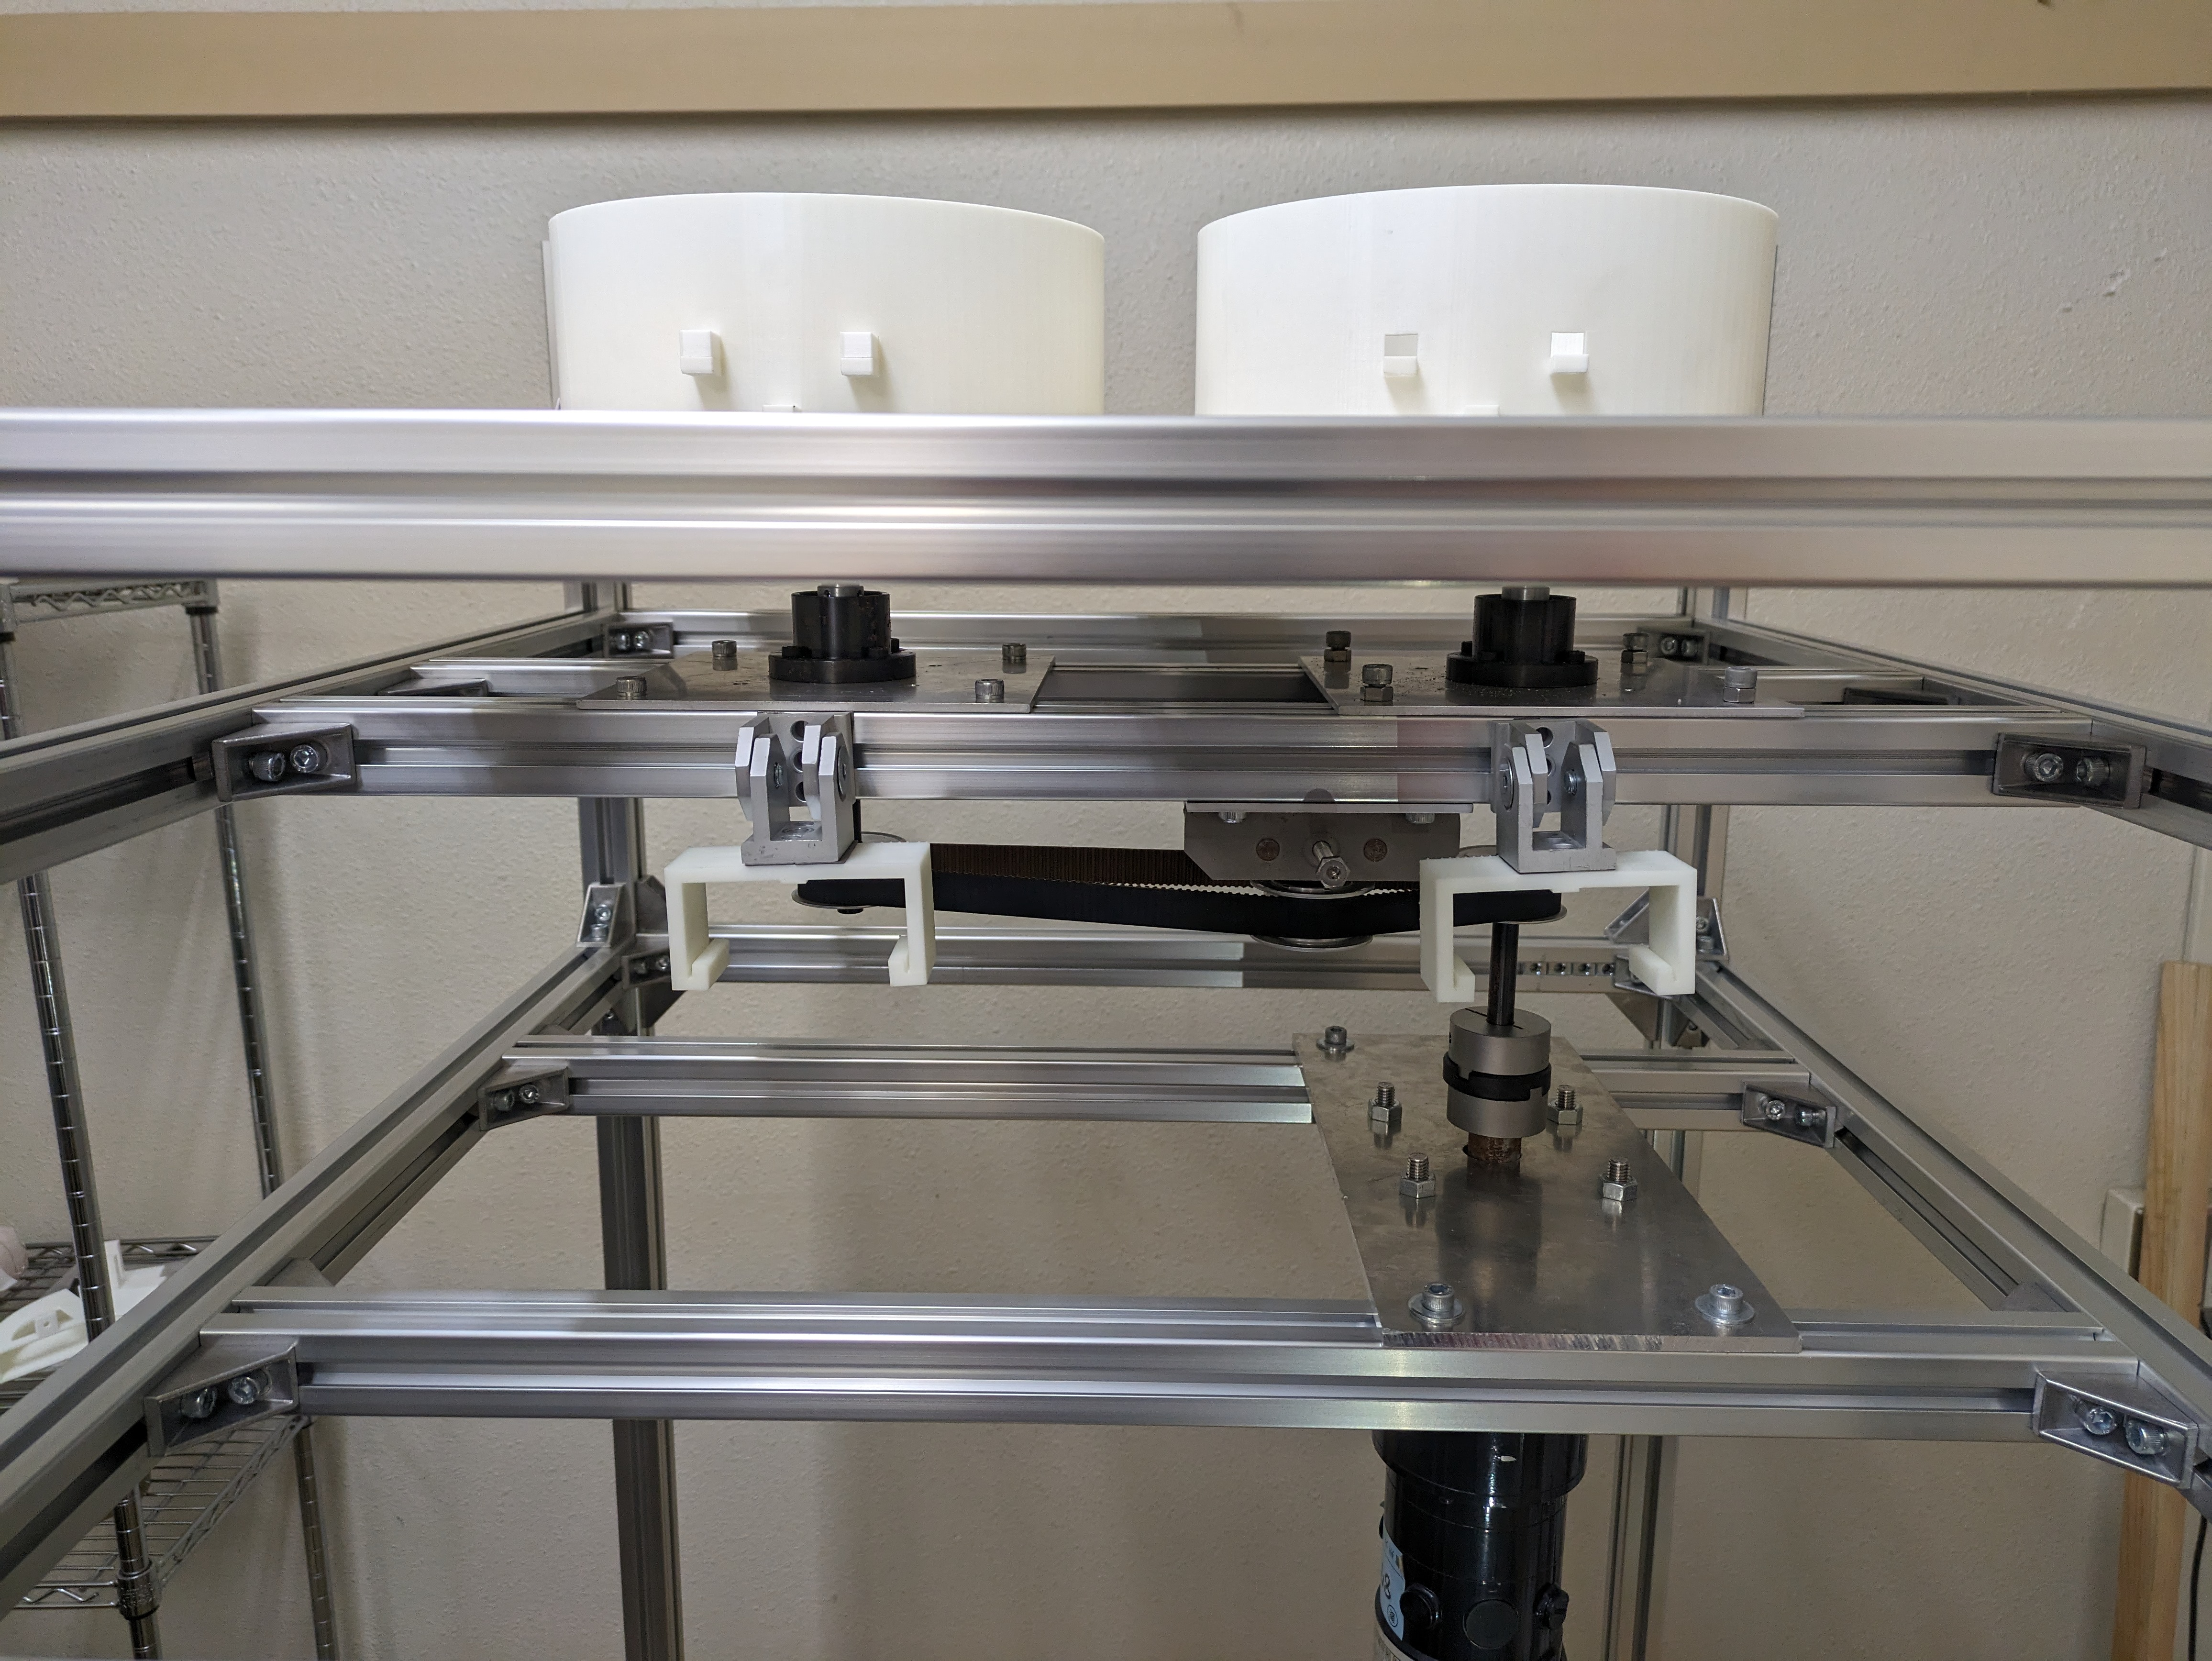
\includegraphics[width=0.9\linewidth]{figures/entire.jpg}
            \subcaption{Entire mechanism}
        \end{minipage}
        \begin{minipage}[t]{0.45\linewidth}
            \centering
            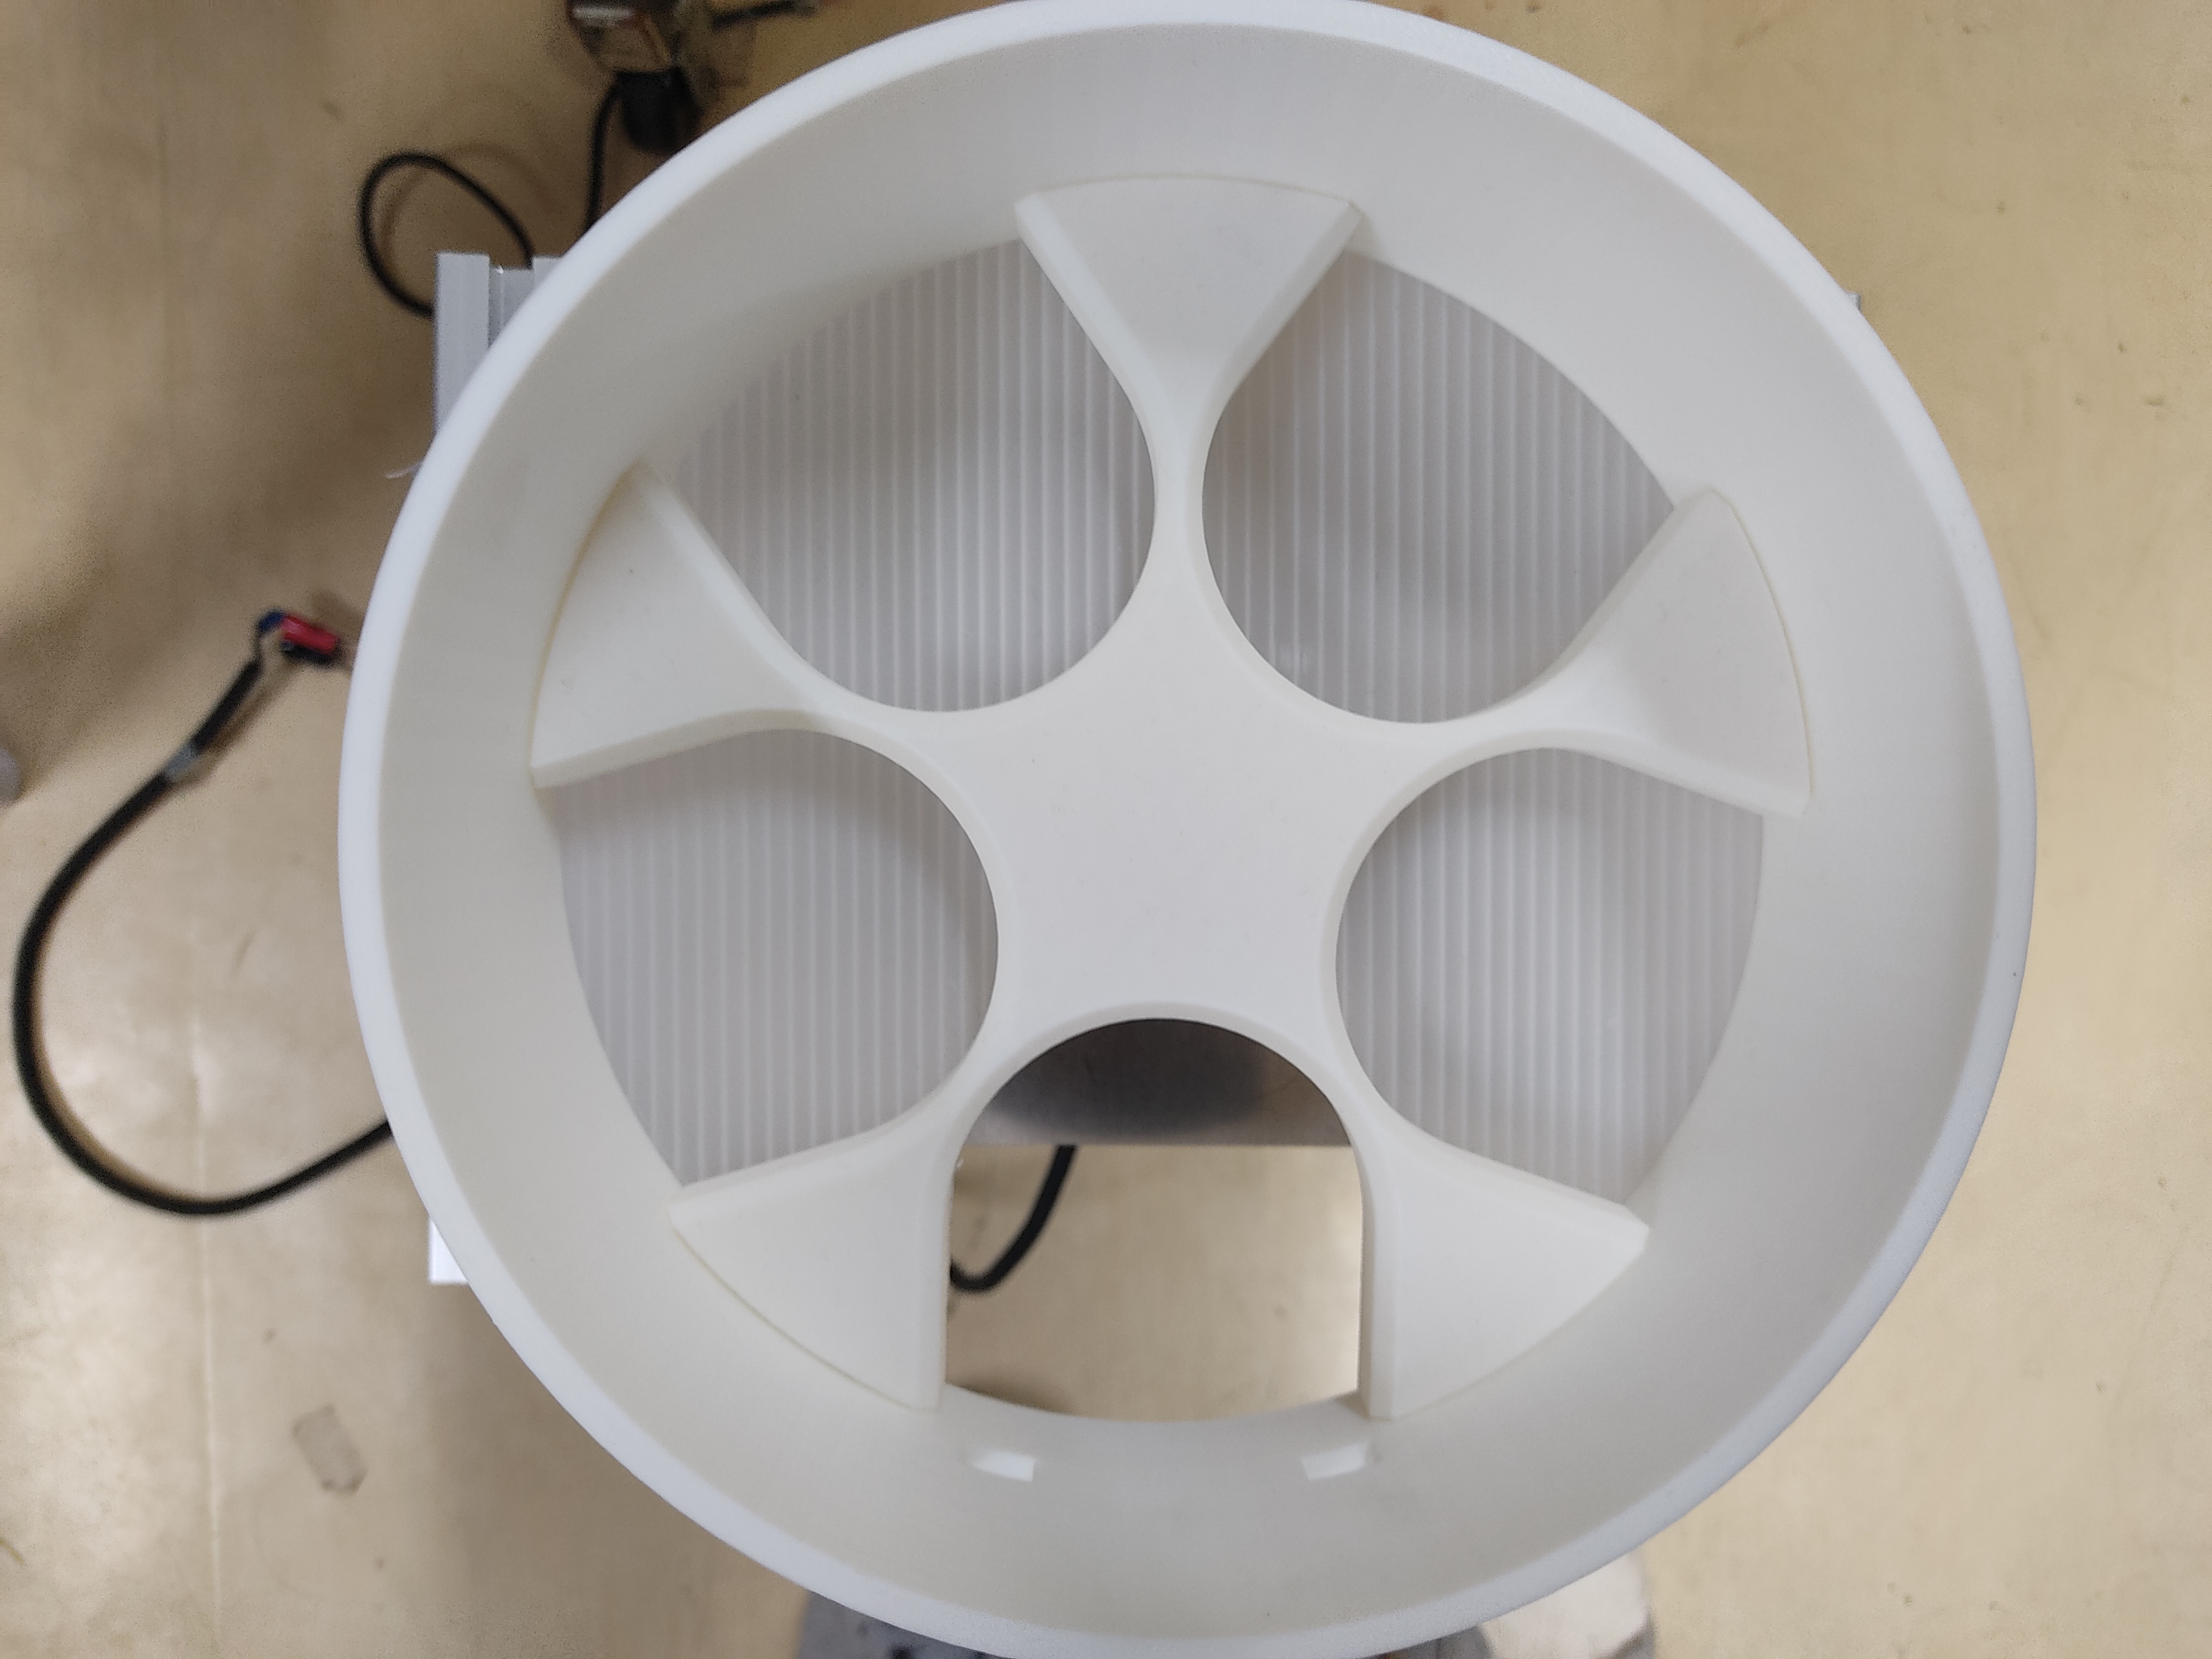
\includegraphics[width=0.9\linewidth]{figures/rotary.jpg}
            \subcaption{Rotary part}
        \end{minipage}
        \caption{Ejection mechanism}
        \label{fig:rotationpart}
    \end{figure}


\subsection{部品の向きを変える機構}
    Fig.\ref{fig:rotationpart}の部品を1つずつ排出する機構では部品が倒れた状態で排出されるため,Fig.\ref{fig:suberidai}のような部品の向きを変える機構が必要である.この部分に部品が入ると,下に排出される際には縦になるように排出される.
    % \vspace{-1zh}
    \begin{figure}[tbp]
        \centering
        \begin{minipage}[t]{0.3\linewidth}
            \centering
            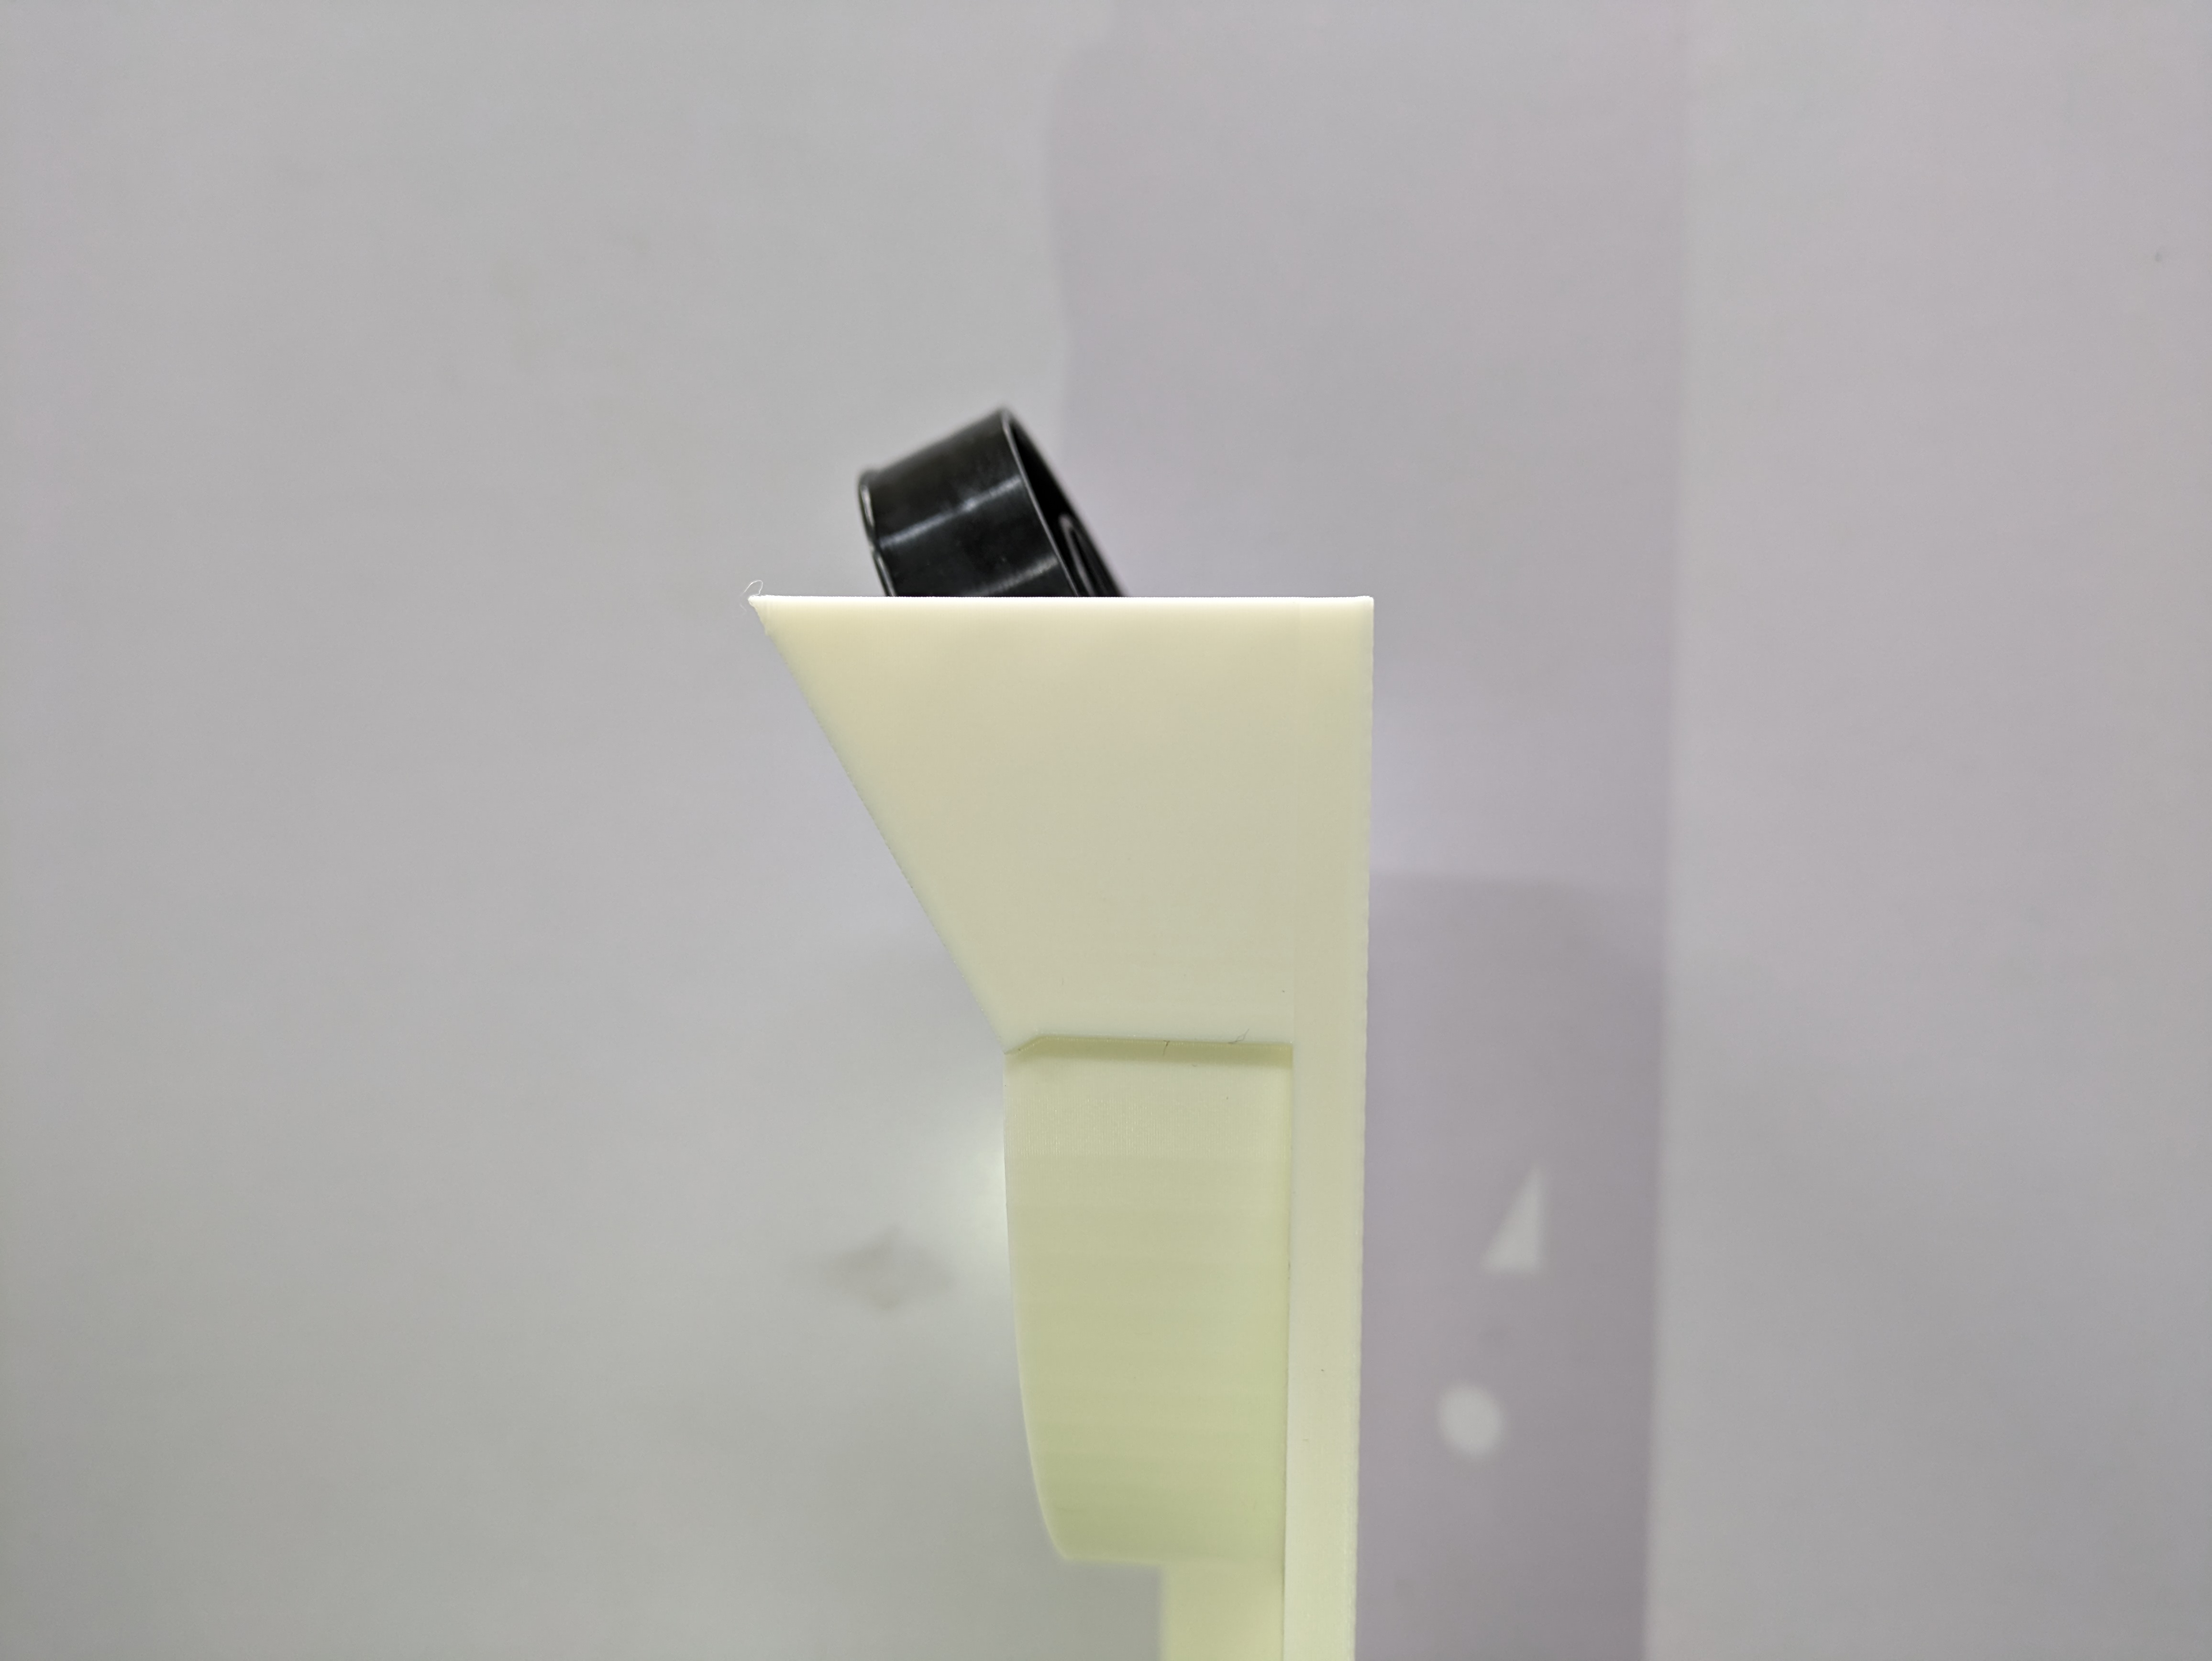
\includegraphics[width=0.9\linewidth]{figures/mukikae_yoko.jpg}
            \subcaption{Side view}
        \end{minipage}
        \begin{minipage}[t]{0.3\linewidth}
            \centering
            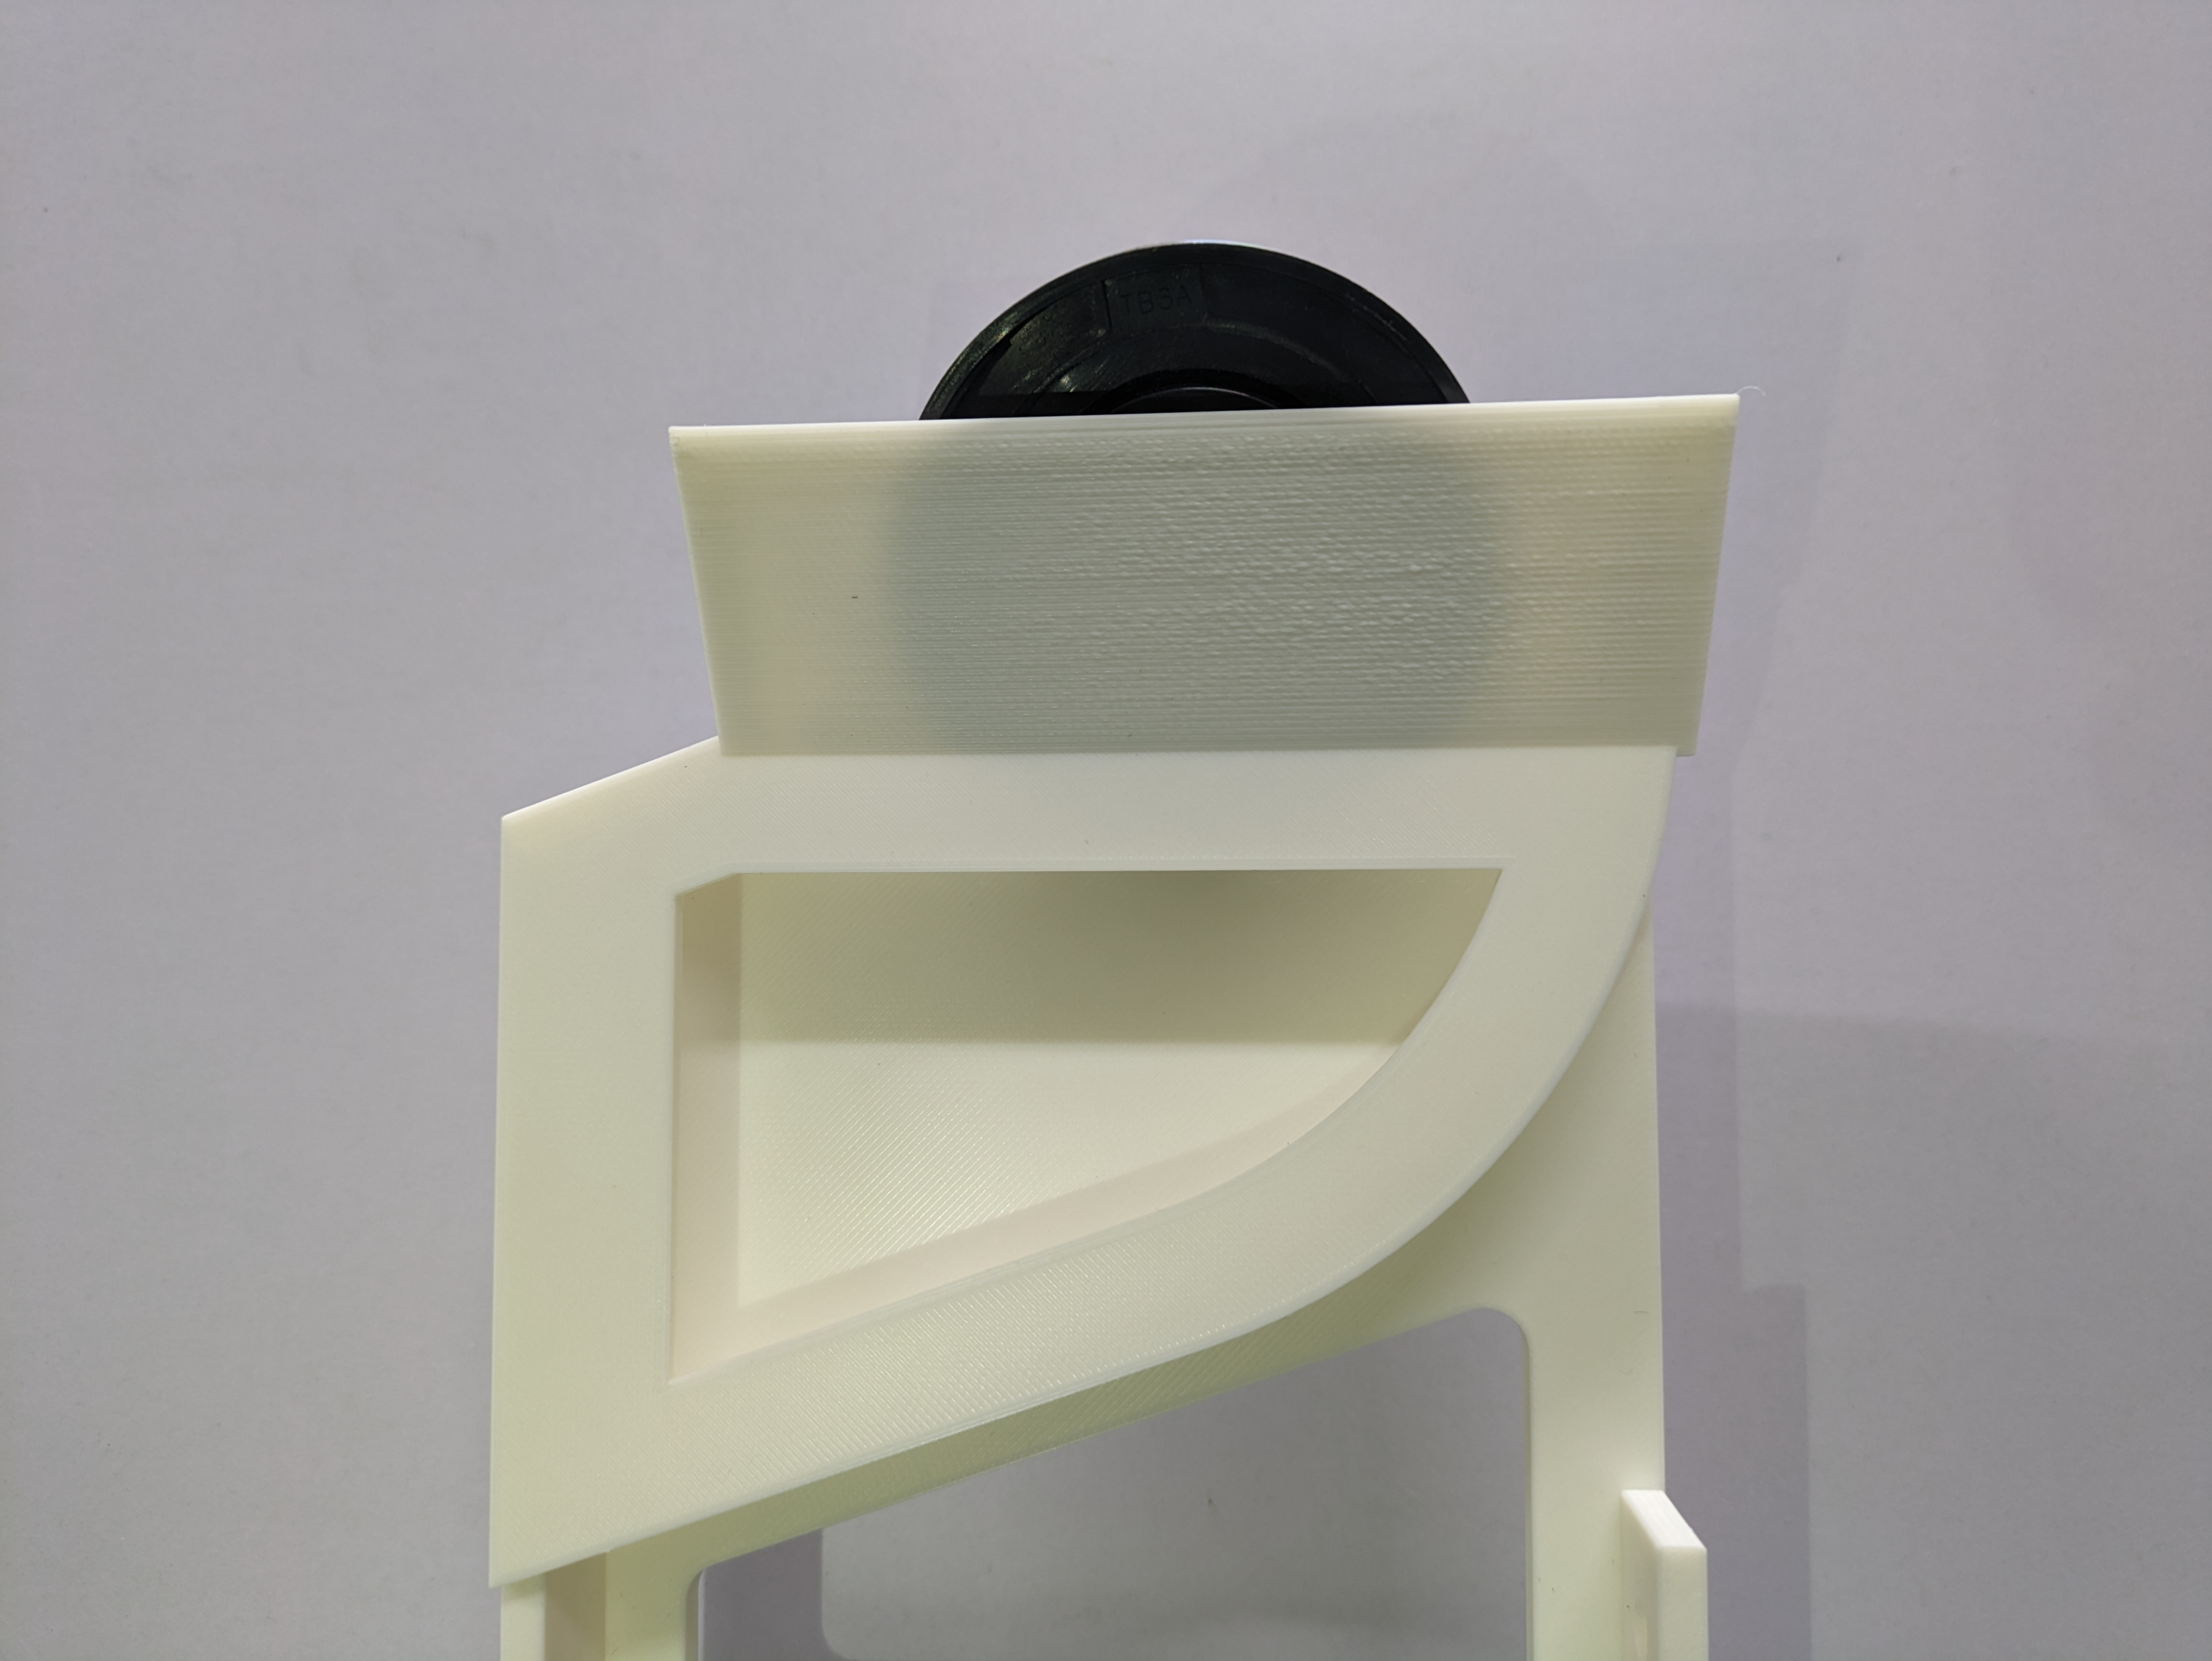
\includegraphics[width=0.9\linewidth]{figures/mukike_syoumen.jpg}
            \subcaption{Front view}
        \end{minipage}
        \begin{minipage}[t]{0.3\linewidth}
            \centering
            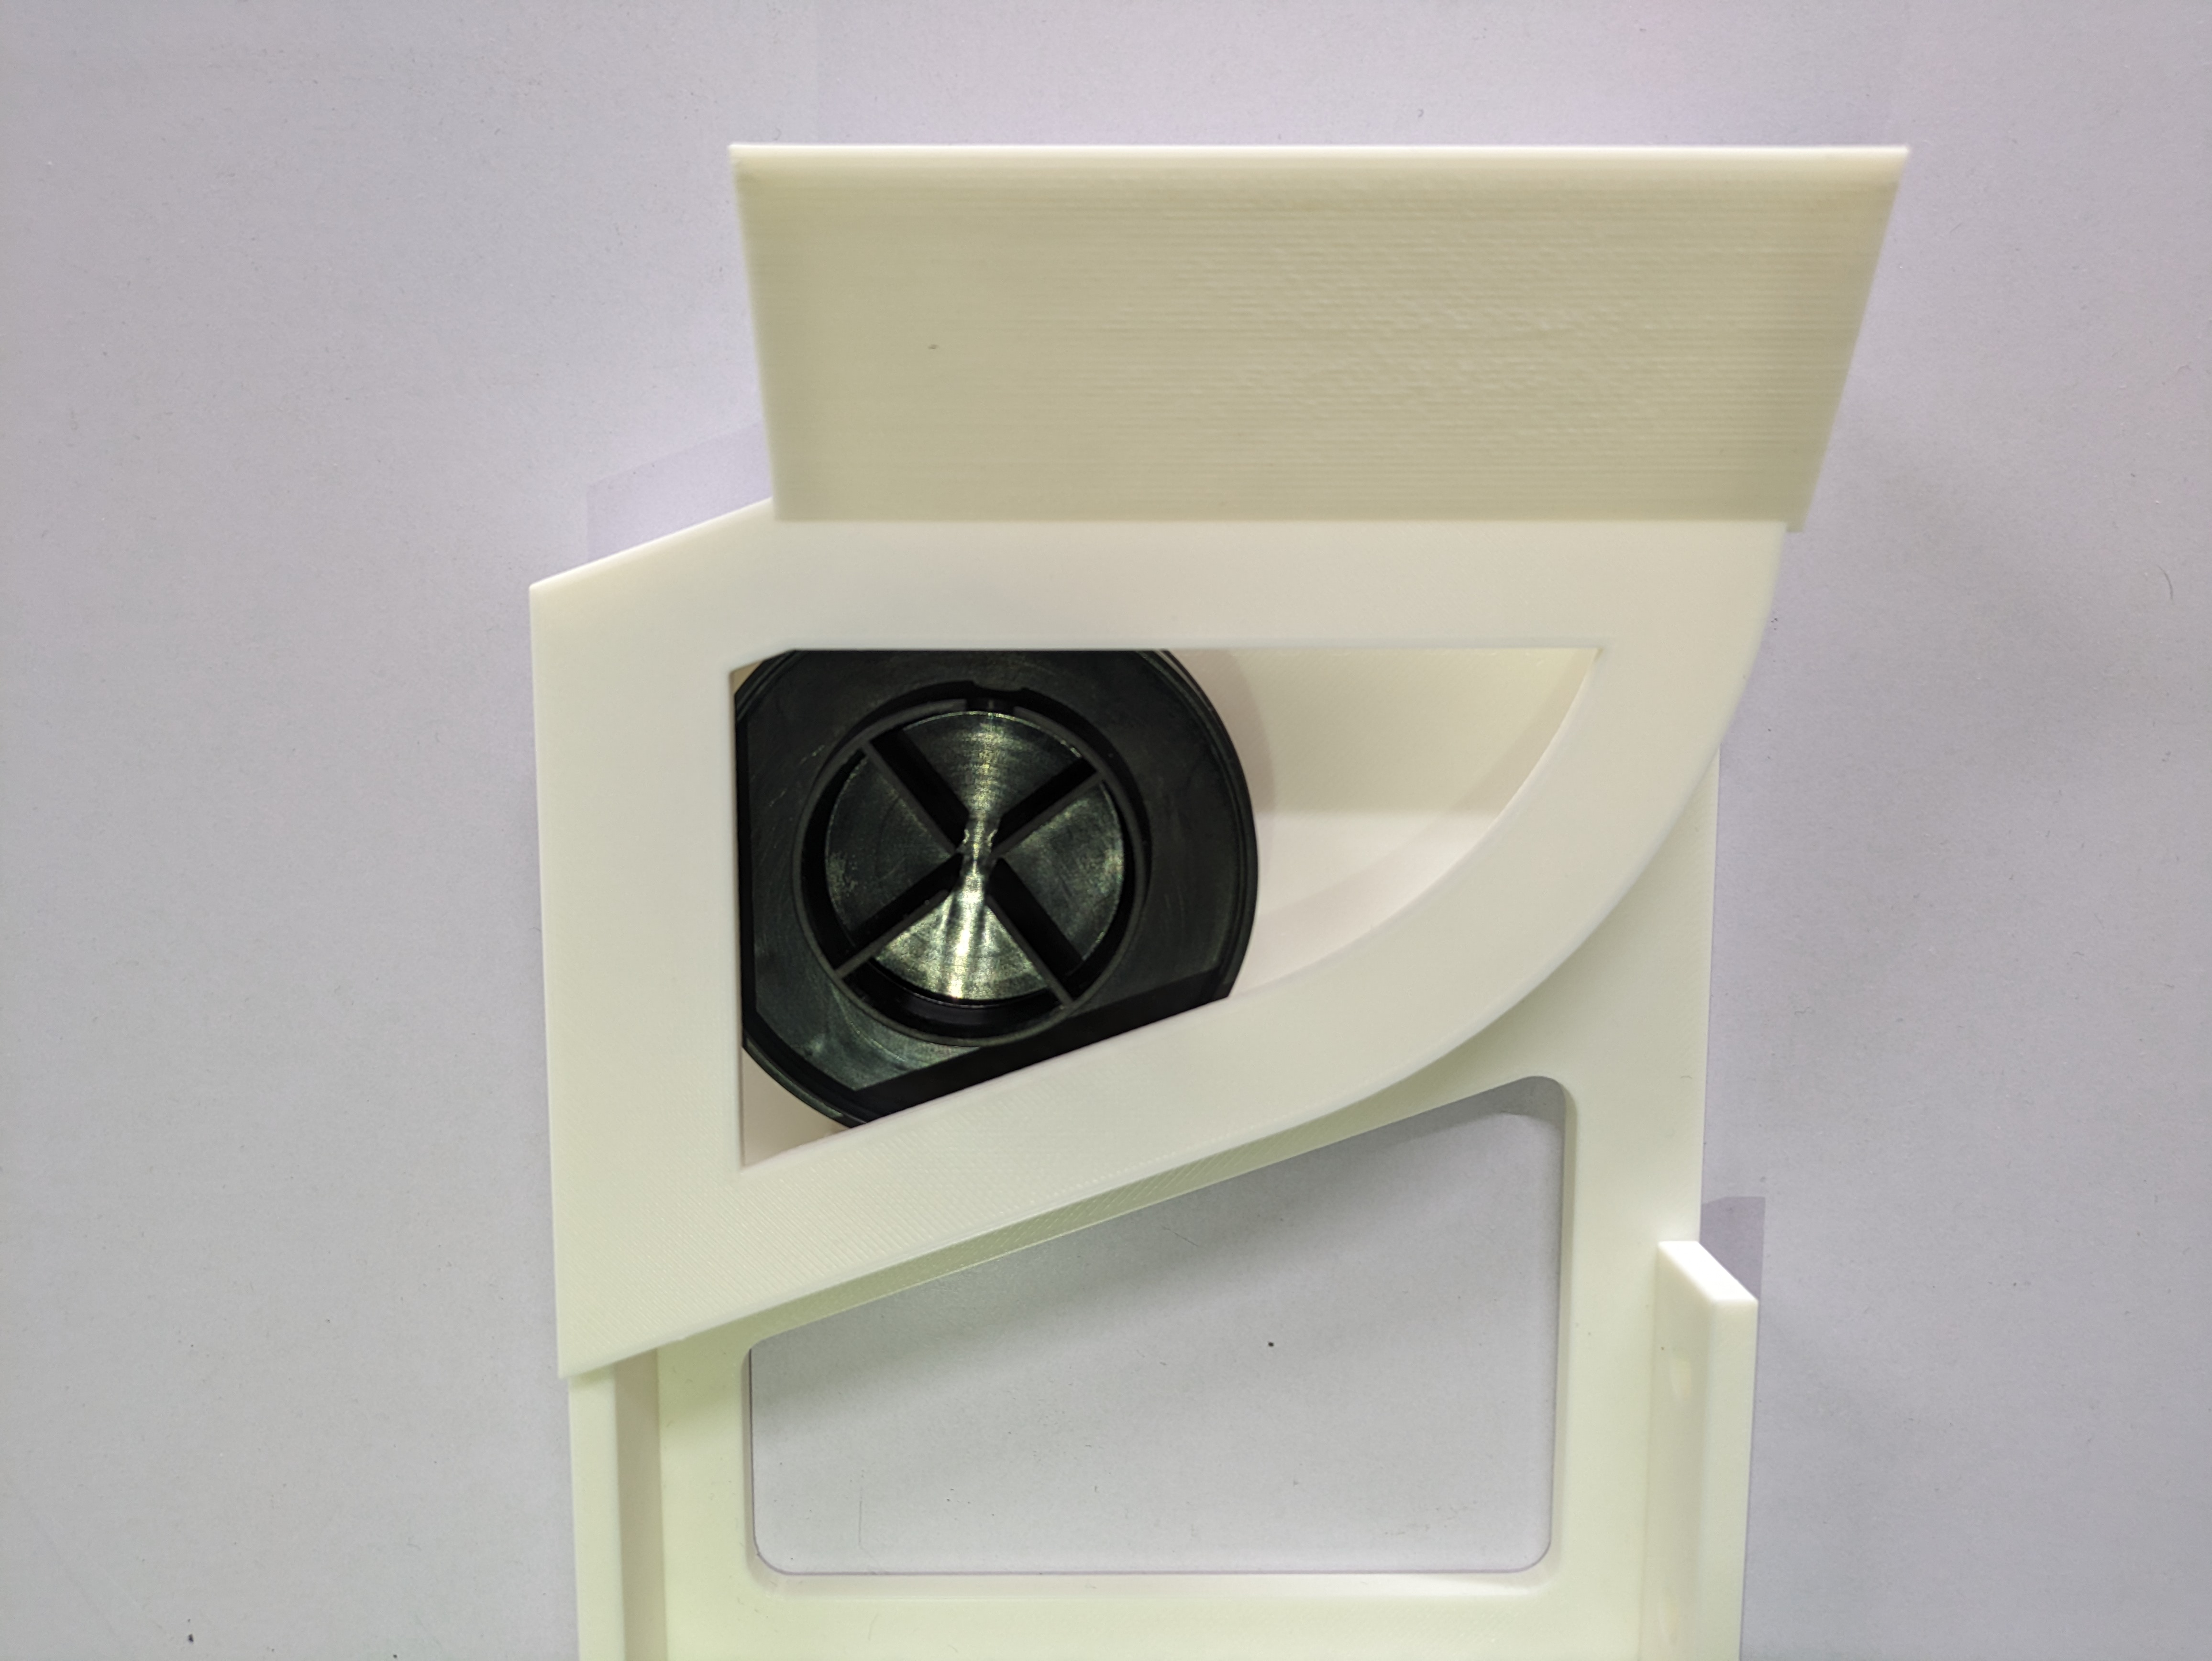
\includegraphics[width=0.9\linewidth]{figures/mukikae_syoumen_done.jpg}
            \subcaption{Diagonal view}
        \end{minipage}
        \caption{Alignment structure}
        \label{fig:suberidai}
    \end{figure}
    % \vspace{-1zh}
\subsection{部品の表裏の判別}
    判別すべき対象は部品2種類の表裏,計4種類である.部品
    判別のためのアルゴリズムとして YOLOv5\cite{ref:DBLP:journals/corr/ZhouGW17a} を用いる.

    YOLOv5 は機械学習を用いた物体検出のためのアルゴ
    リズムである.機械学習を用いた物体検出には様々な手法
    があるが,YOLOv5 はその中でも処理速度が高速な手法で
    ある.今回は判別すべきものが2種類4パターンと少ないため,判
    別能力より処理速度を重視した YOLOv5 を採用した.

\subsection{部品をスタックする機構}
    全体像をFig.\ref{fig:detectarea}に示す.
    この部分でYOLOv5による表裏判別をするため,カメラで見ても部品がスタックされていることがわかるようにする.カメラで内部を見れるように上面には低反射ガラスを使用する.以前はアクリル板を使っていたが光源が映り込み誤検知の原因となったので,低反射ガラスに変更した.

    また工場での日照の変化を考えて,光源を一定にするためにアルミ製の箱で全体を囲み,内部に照明を設置する.


    \begin{figure}[htbp]
        \centering
        \begin{minipage}[t]{0.45\linewidth}
            \centering
            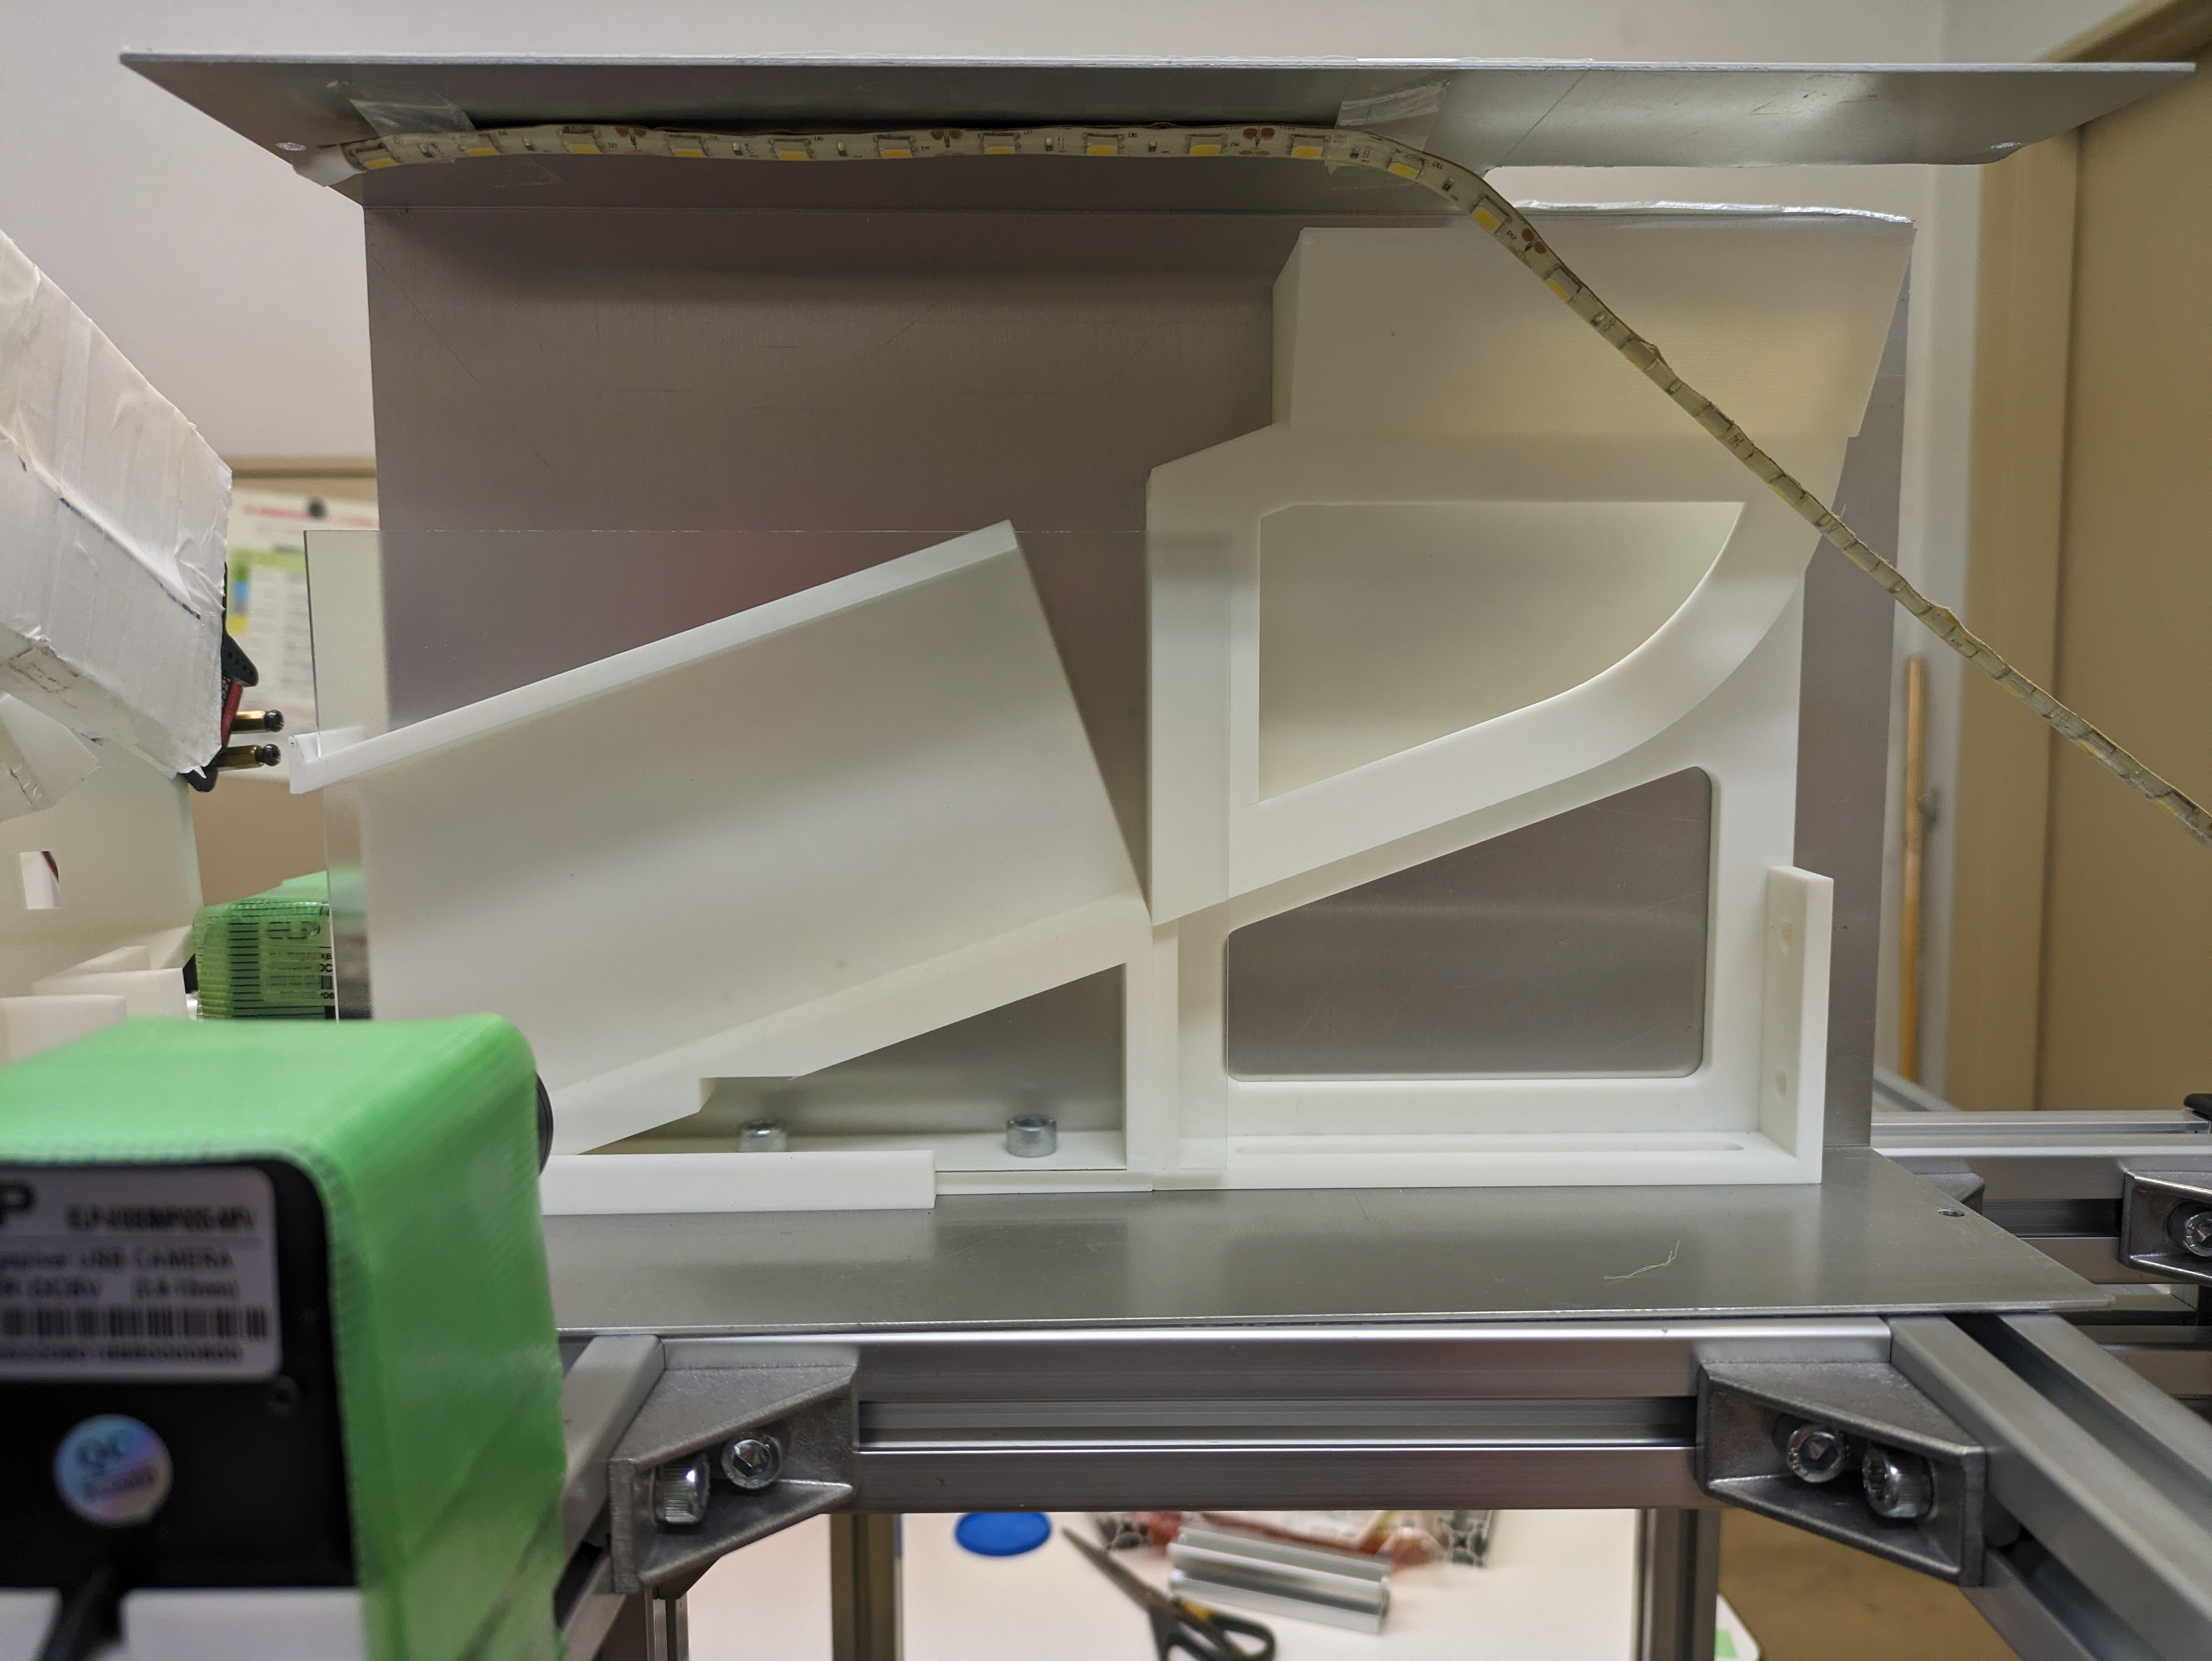
\includegraphics[width=0.9\linewidth]{figures/strip_box.jpg}
            \subcaption{Detect area}
        \end{minipage}
        \begin{minipage}[t]{0.45\linewidth}
            \centering
            \includegraphics[width=0.9\linewidth]{figures/box.jpg}
            \subcaption{Overview of detect area}
        \end{minipage}
        \caption{Stuck structure}
        \label{fig:detectarea}
    \end{figure}
    \vspace*{-1\zh}

\subsection{部品を反転させる機構}

    ArduinoとPCと光透過センサを用いて部品を検知するシステムを作成する.光透過センサが部品を検知したら,ArduinoからPCに信号を送り,PC内のYOLOv5で部品の表裏を判別する.その結果によってサーボモータを動かし,部品を反転させる.

    \section{結言}
\subsection{本研究のまとめ}
    本研究では緒言で述べた問題点を解決するために,部品を一つずつ排出する機構,部品の向きを変える機構,部品を反転させる機構,部品を検知するシステムを設計した.さらに各機構に改善を加えた.
\subsection{今後の方針}
    全体を通しての動作確認を行う.

    \subfile{sections/references.tex}

\end{document}